% Editable native annotations around unchanged verified IDE photographs.
\par
\begin{figure}[htbp]
\centering
\newsavebox{\MARSmatmulscalarregistersBox}
\sbox{\MARSmatmulscalarregistersBox}{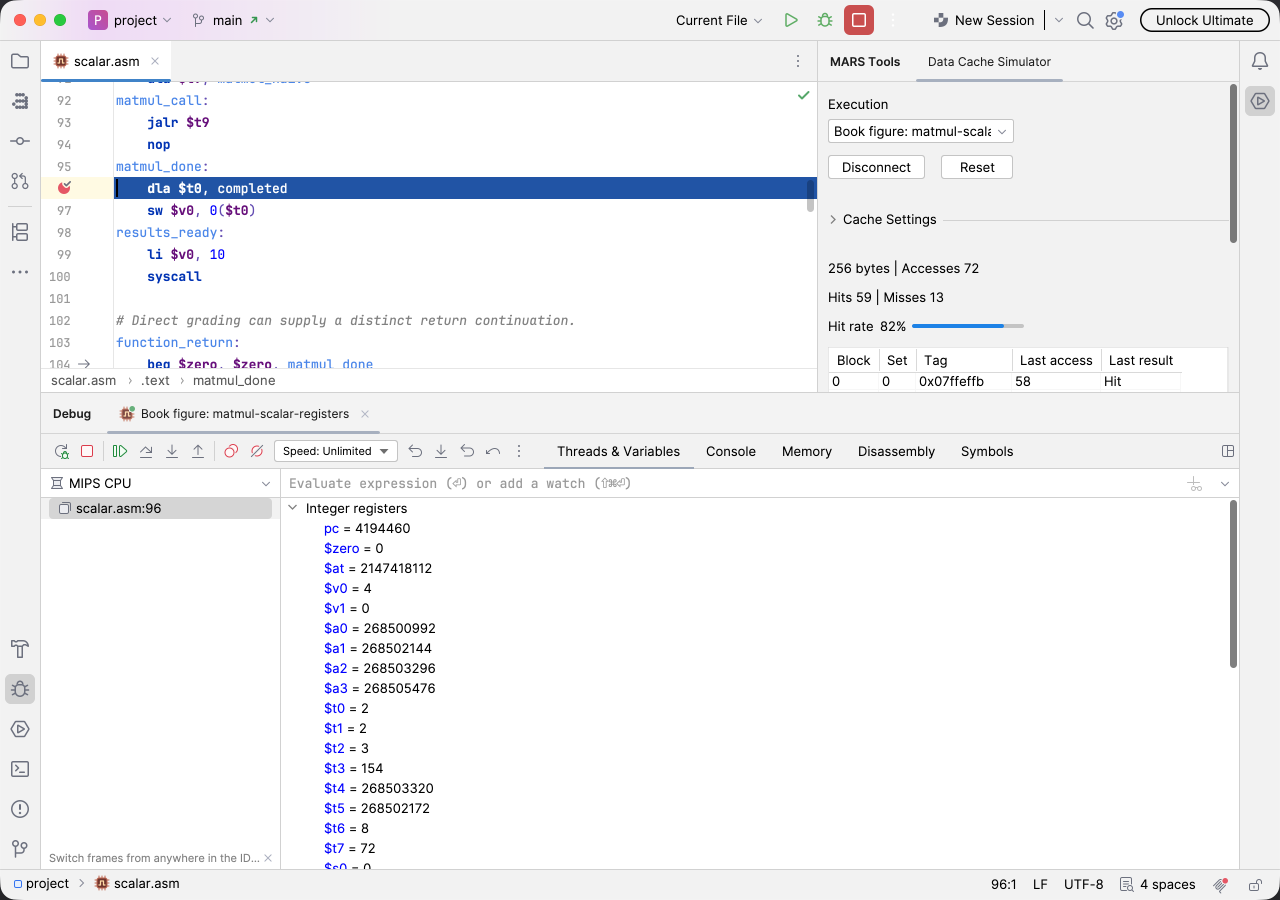
\includegraphics[artifact]{packages/022-blocked-matmul/captures/f01/registers.png}}
\newsavebox{\MARSmatmulscalarleftBox}
\sbox{\MARSmatmulscalarleftBox}{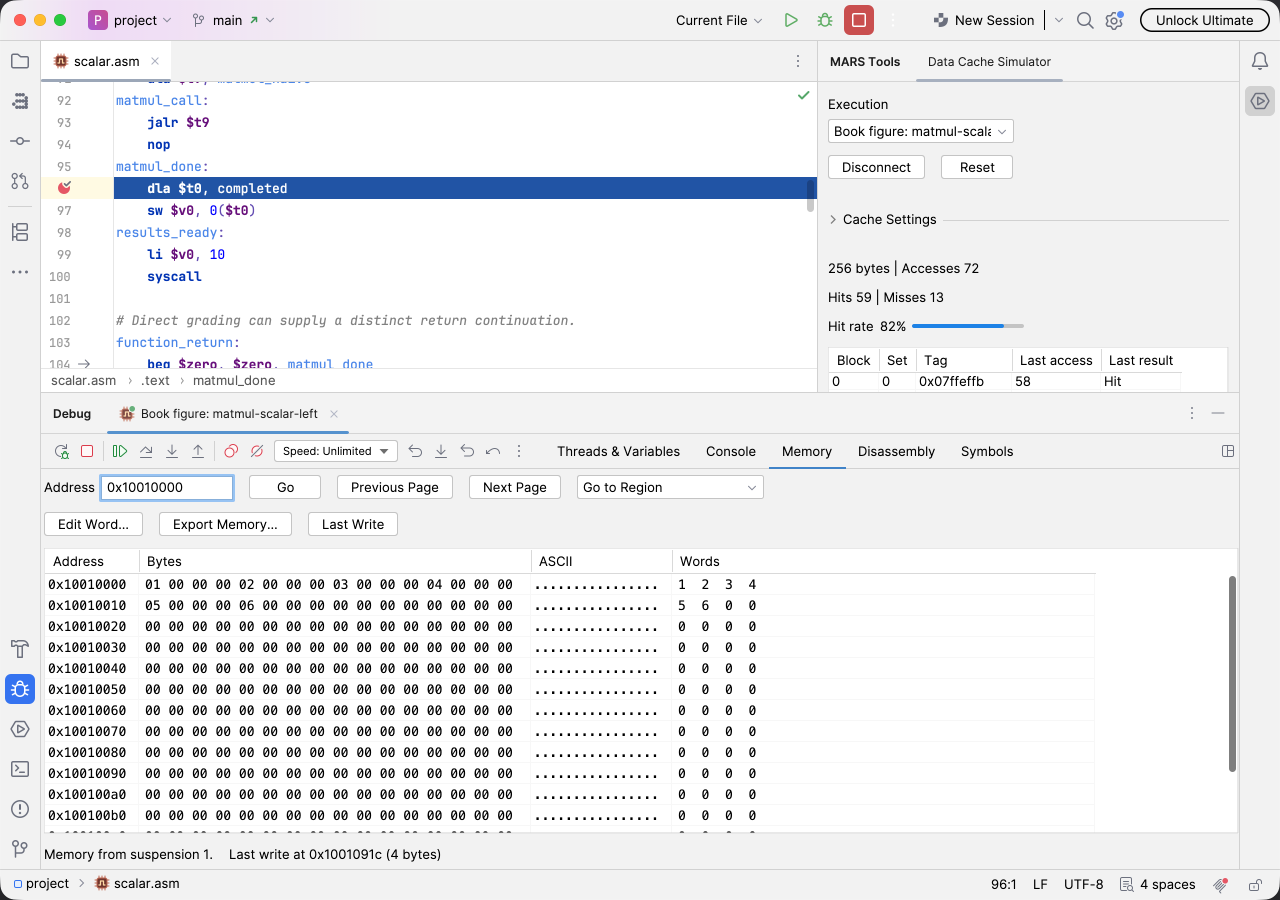
\includegraphics[artifact]{packages/022-blocked-matmul/captures/f01/left.png}}
\newsavebox{\MARSmatmulscalarrightBox}
\sbox{\MARSmatmulscalarrightBox}{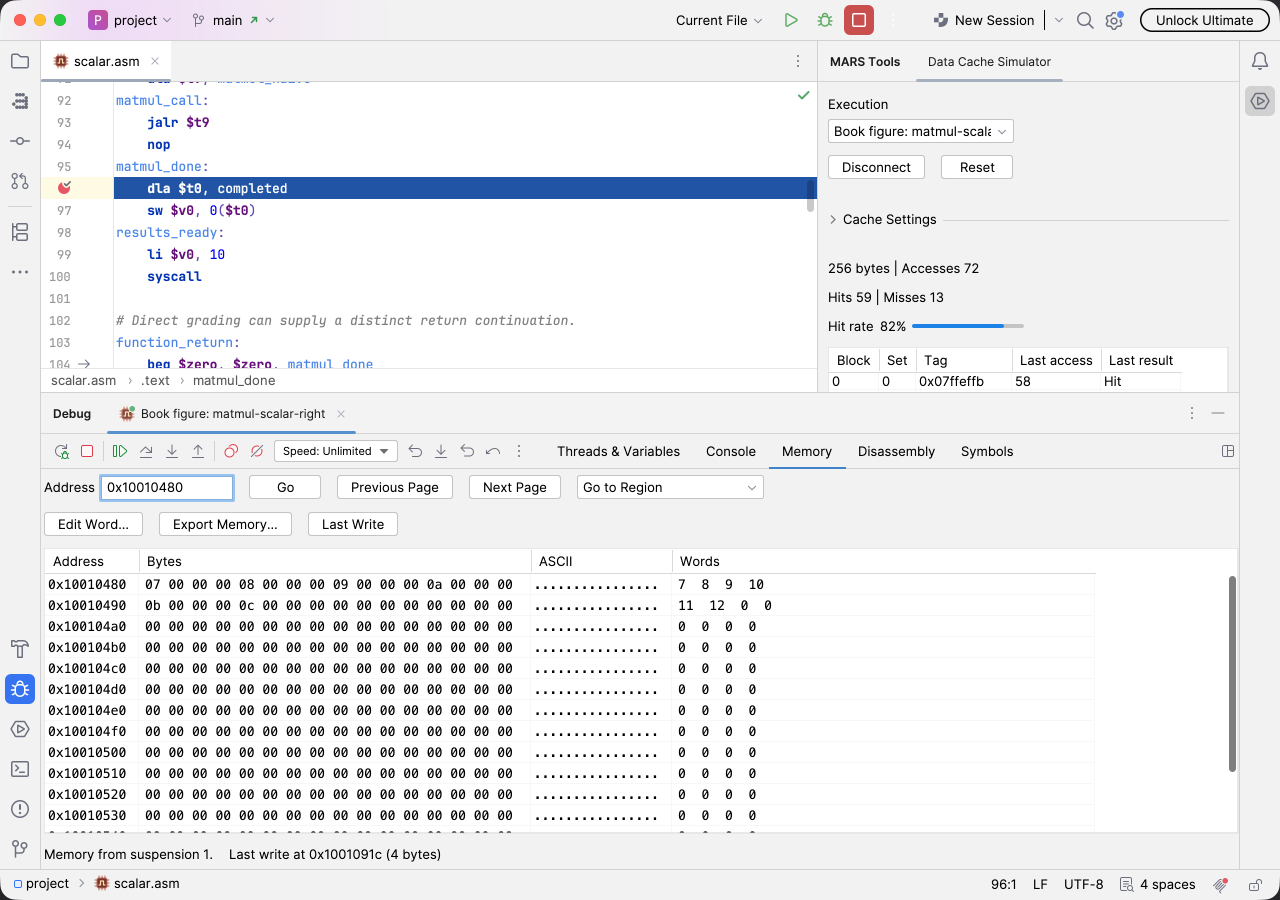
\includegraphics[artifact]{packages/022-blocked-matmul/captures/f01/right.png}}
\newsavebox{\MARSmatmulscalarproductBox}
\sbox{\MARSmatmulscalarproductBox}{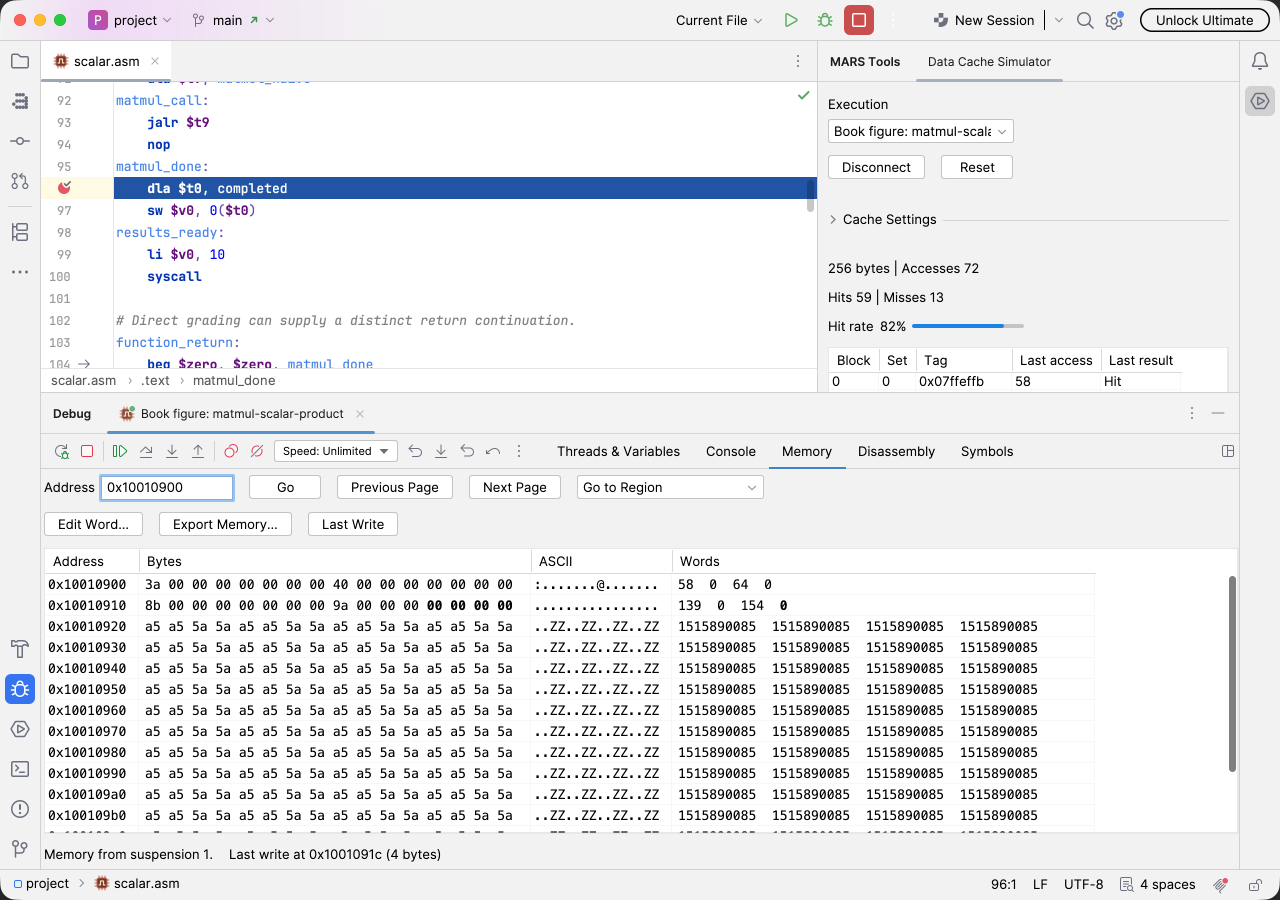
\includegraphics[artifact]{packages/022-blocked-matmul/captures/f01/product.png}}
\newsavebox{\MARSmatmulscalarcallerBox}
\sbox{\MARSmatmulscalarcallerBox}{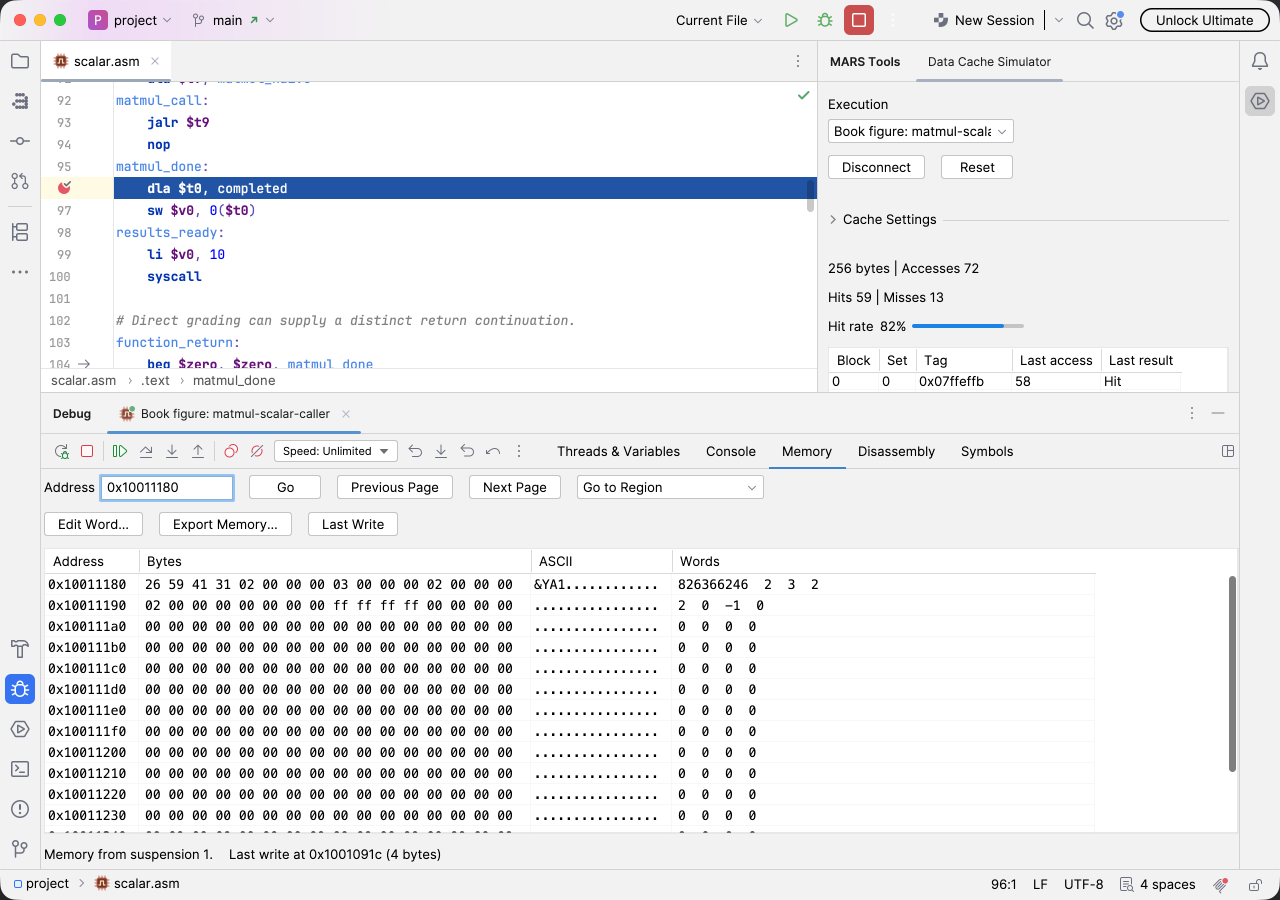
\includegraphics[artifact]{packages/022-blocked-matmul/captures/f01/caller.png}}
\edef\MARSmatmulscalarsourceLeft{\the\dimexpr0.036718750\wd\MARSmatmulscalarregistersBox\relax}
\edef\MARSmatmulscalarsourceBottom{\the\dimexpr0.774444444\ht\MARSmatmulscalarregistersBox\relax}
\edef\MARSmatmulscalarsourceRight{\the\dimexpr0.713281250\wd\MARSmatmulscalarregistersBox\relax}
\edef\MARSmatmulscalarsourceTop{\the\dimexpr0.170000000\ht\MARSmatmulscalarregistersBox\relax}
\edef\MARSmatmulscalarregistersLeft{\the\dimexpr0.246093750\wd\MARSmatmulscalarregistersBox\relax}
\edef\MARSmatmulscalarregistersBottom{\the\dimexpr0.334444444\ht\MARSmatmulscalarregistersBox\relax}
\edef\MARSmatmulscalarregistersRight{\the\dimexpr0.553906250\wd\MARSmatmulscalarregistersBox\relax}
\edef\MARSmatmulscalarregistersTop{\the\dimexpr0.640000000\ht\MARSmatmulscalarregistersBox\relax}
\edef\MARSmatmulscalarleftLeft{\the\dimexpr0.034375000\wd\MARSmatmulscalarleftBox\relax}
\edef\MARSmatmulscalarleftBottom{\the\dimexpr0.311111111\ht\MARSmatmulscalarleftBox\relax}
\edef\MARSmatmulscalarleftRight{\the\dimexpr0.584375000\wd\MARSmatmulscalarleftBox\relax}
\edef\MARSmatmulscalarleftTop{\the\dimexpr0.608888889\ht\MARSmatmulscalarleftBox\relax}
\edef\MARSmatmulscalarrightLeft{\the\dimexpr0.034375000\wd\MARSmatmulscalarrightBox\relax}
\edef\MARSmatmulscalarrightBottom{\the\dimexpr0.311111111\ht\MARSmatmulscalarrightBox\relax}
\edef\MARSmatmulscalarrightRight{\the\dimexpr0.584375000\wd\MARSmatmulscalarrightBox\relax}
\edef\MARSmatmulscalarrightTop{\the\dimexpr0.608888889\ht\MARSmatmulscalarrightBox\relax}
\edef\MARSmatmulscalarproductLeft{\the\dimexpr0.034375000\wd\MARSmatmulscalarproductBox\relax}
\edef\MARSmatmulscalarproductBottom{\the\dimexpr0.311111111\ht\MARSmatmulscalarproductBox\relax}
\edef\MARSmatmulscalarproductRight{\the\dimexpr0.584375000\wd\MARSmatmulscalarproductBox\relax}
\edef\MARSmatmulscalarproductTop{\the\dimexpr0.608888889\ht\MARSmatmulscalarproductBox\relax}
\edef\MARSmatmulscalarcallerLeft{\the\dimexpr0.034375000\wd\MARSmatmulscalarcallerBox\relax}
\edef\MARSmatmulscalarcallerBottom{\the\dimexpr0.311111111\ht\MARSmatmulscalarcallerBox\relax}
\edef\MARSmatmulscalarcallerRight{\the\dimexpr0.584375000\wd\MARSmatmulscalarcallerBox\relax}
\edef\MARSmatmulscalarcallerTop{\the\dimexpr0.608888889\ht\MARSmatmulscalarcallerBox\relax}
\begin{tikzpicture}[alt={Six annotated details at matmul_done show return four, left rows one two three and four five six, right rows seven eight, nine ten and eleven twelve, output doublewords 58 64 139 154, and a completed word still minus one.}]
\node[anchor=north west,inner sep=0,font=\small\bfseries] (source-title) at (6mm,0) {Next instruction at this boundary};
\node[anchor=north west,inner sep=0] (source) at ([yshift=-1mm]source-title.south west) {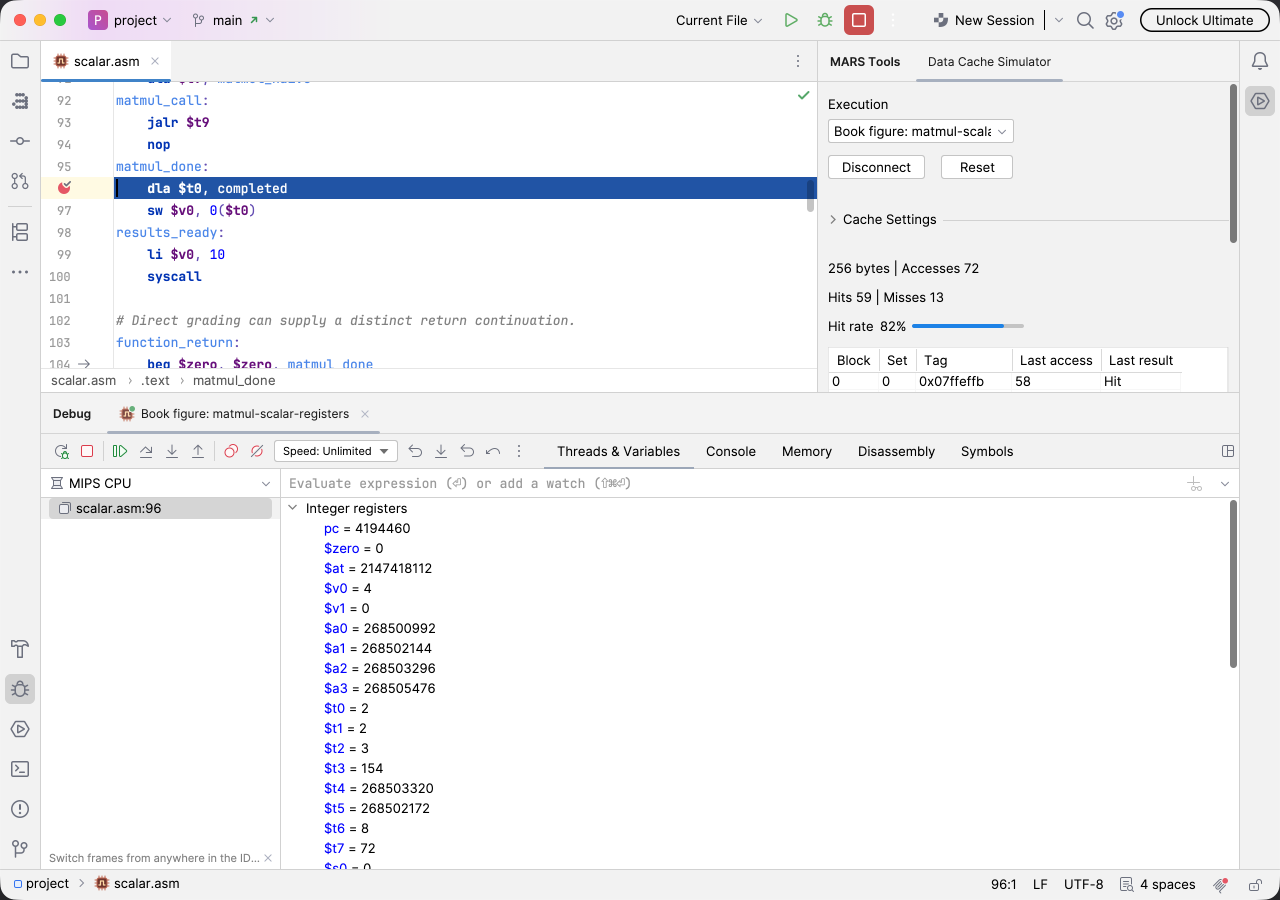
\includegraphics[width=0.54\linewidth,artifact,trim={\MARSmatmulscalarsourceLeft{} \MARSmatmulscalarsourceBottom{} \MARSmatmulscalarsourceRight{} \MARSmatmulscalarsourceTop{}},clip]{packages/022-blocked-matmul/captures/f01/registers.png}};
\begin{scope}[shift={(source.south west)},x={($(source.south east)-(source.south west)$)},y={($(source.north west)-(source.south west)$)}]
\draw[black,line width=0.7pt] (0.215625000,0.080000000) rectangle (0.750000000,0.520000000);
\node[draw=black,fill=white,circle,inner sep=1.5pt,font=\footnotesize] at ($(0.215625000,0.520000000)+(-3mm,0)$) {1};
\end{scope}
\node[anchor=north west,inner sep=0,font=\small\bfseries] (registers-title) at (0.58\linewidth,0 |- source-title.north) {Register value at this boundary};
\node[anchor=north west,inner sep=0] (registers) at ([yshift=-1mm]registers-title.south west) {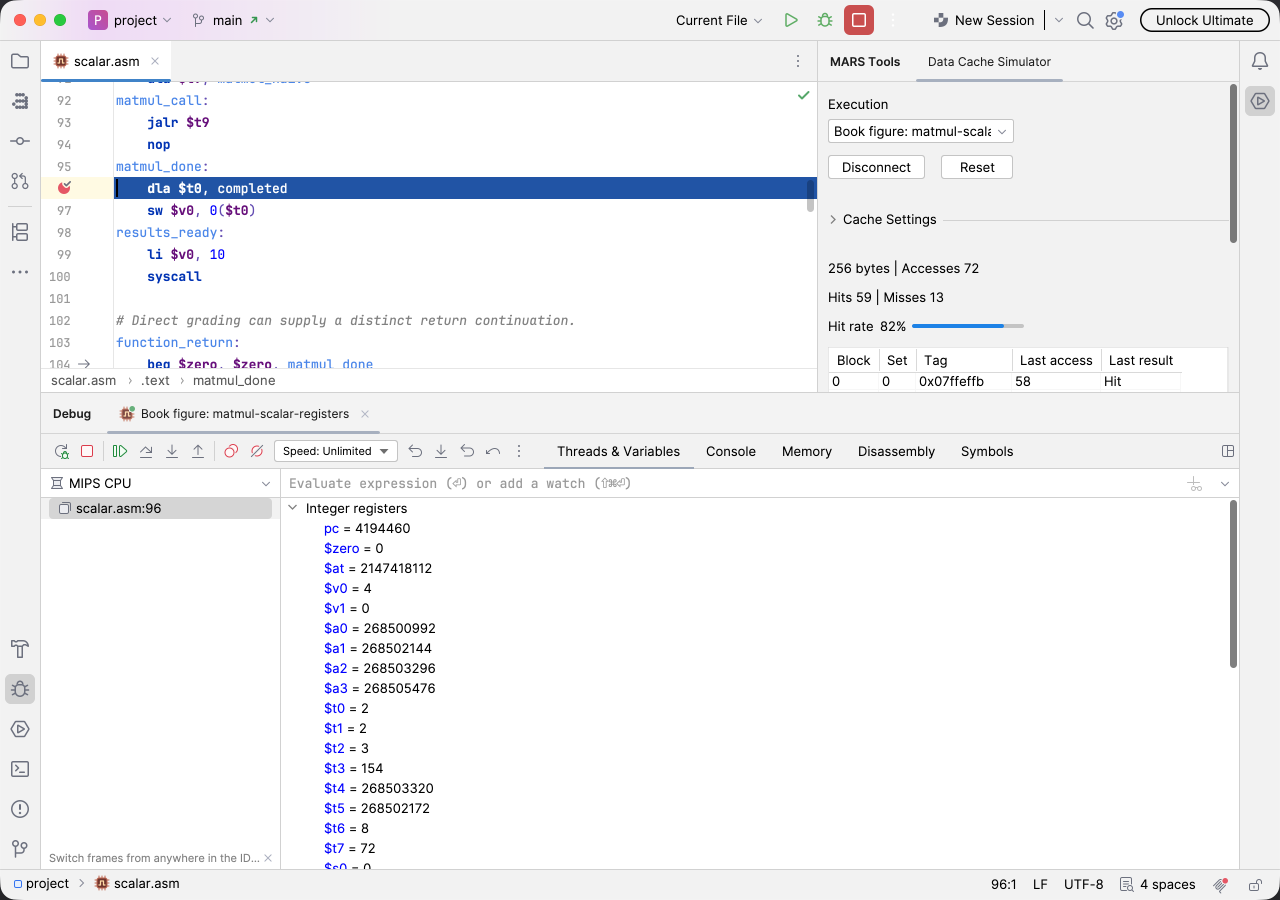
\includegraphics[width=0.42\linewidth,artifact,trim={\MARSmatmulscalarregistersLeft{} \MARSmatmulscalarregistersBottom{} \MARSmatmulscalarregistersRight{} \MARSmatmulscalarregistersTop{}},clip]{packages/022-blocked-matmul/captures/f01/registers.png}};
\begin{scope}[shift={(registers.south west)},x={($(registers.south east)-(registers.south west)$)},y={($(registers.north west)-(registers.south west)$)}]
\draw[black,line width=0.7pt] (0.023437500,0.043478261) rectangle (0.226562500,0.913043478);
\node[draw=black,fill=white,circle,inner sep=1.5pt,font=\footnotesize] at ($(0.023437500,0.913043478)+(-3mm,0)$) {2};
\end{scope}
\node[anchor=north west,inner sep=0,font=\small\bfseries] (left-title) at ([yshift=-1mm]source.south west) {Left input words};
\node[anchor=north west,inner sep=0] (left) at ([yshift=-1mm]left-title.south west) {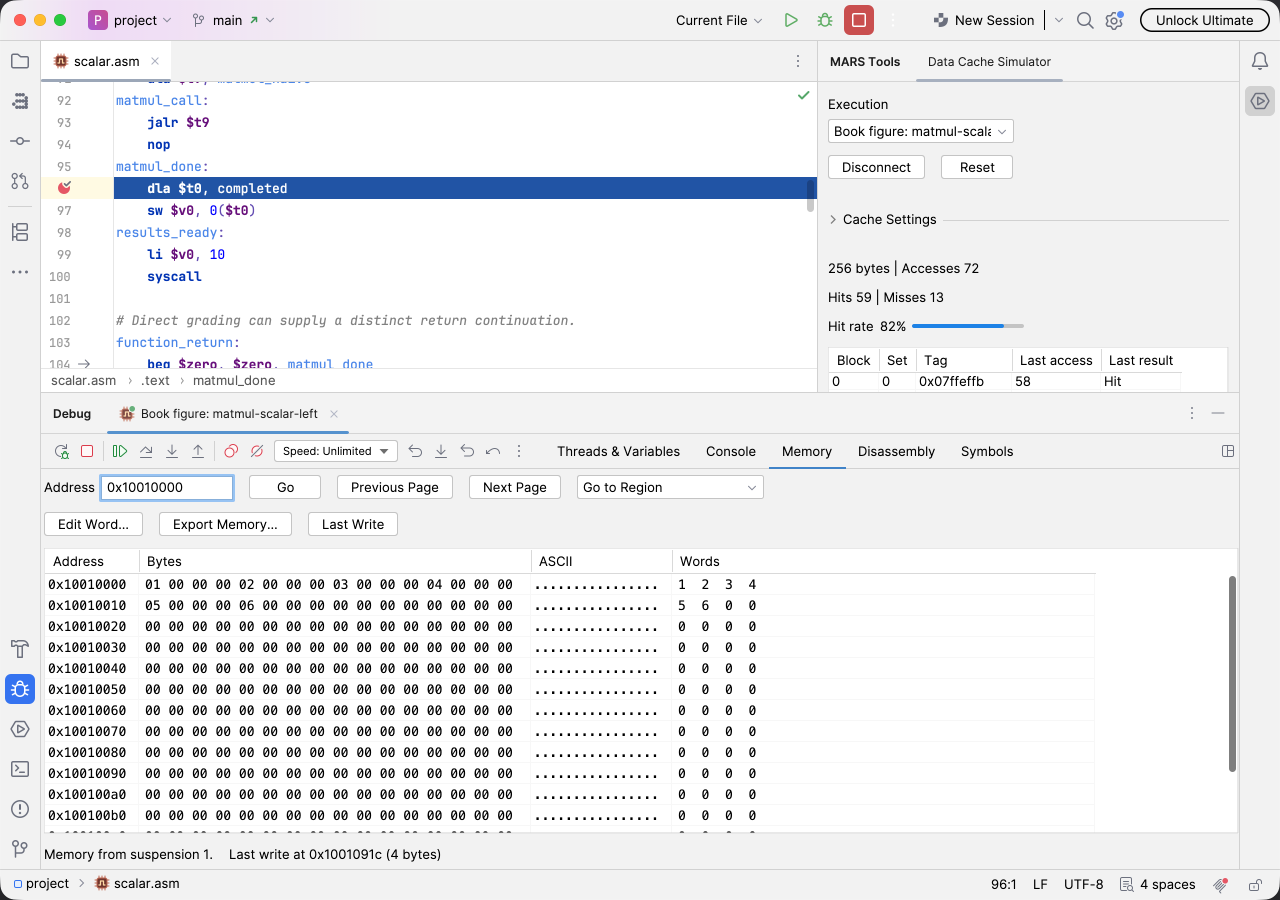
\includegraphics[width=0.84\linewidth,artifact,trim={\MARSmatmulscalarleftLeft{} \MARSmatmulscalarleftBottom{} \MARSmatmulscalarleftRight{} \MARSmatmulscalarleftTop{}},clip]{packages/022-blocked-matmul/captures/f01/left.png}};
\begin{scope}[shift={(left.south west)},x={($(left.south east)-(left.south west)$)},y={($(left.north west)-(left.south west)$)}]
\draw[black,line width=0.7pt] (0.194672131,0.055555556) rectangle (0.997950820,0.638888889);
\node[draw=black,fill=white,circle,inner sep=1.5pt,font=\footnotesize] at ($(0,0.638888889)+(-3mm,0)$) {3};
\end{scope}
\node[anchor=north west,inner sep=0,font=\small\bfseries] (right-title) at ([yshift=-1mm]left.south west) {Right input words};
\node[anchor=north west,inner sep=0] (right) at ([yshift=-1mm]right-title.south west) {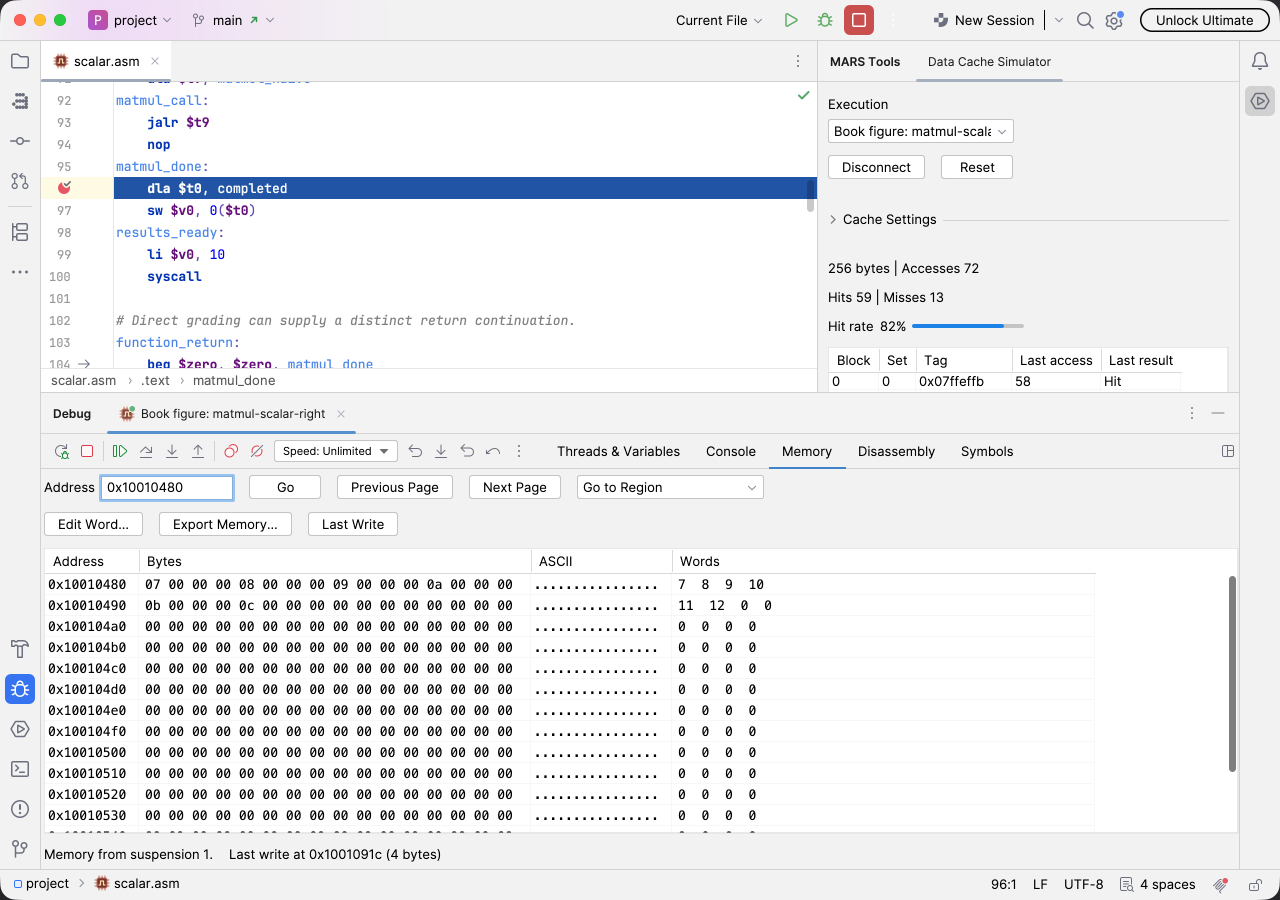
\includegraphics[width=0.84\linewidth,artifact,trim={\MARSmatmulscalarrightLeft{} \MARSmatmulscalarrightBottom{} \MARSmatmulscalarrightRight{} \MARSmatmulscalarrightTop{}},clip]{packages/022-blocked-matmul/captures/f01/right.png}};
\begin{scope}[shift={(right.south west)},x={($(right.south east)-(right.south west)$)},y={($(right.north west)-(right.south west)$)}]
\draw[black,line width=0.7pt] (0.194672131,0.055555556) rectangle (0.997950820,0.638888889);
\node[draw=black,fill=white,circle,inner sep=1.5pt,font=\footnotesize] at ($(0,0.638888889)+(-3mm,0)$) {4};
\end{scope}
\node[anchor=north west,inner sep=0,font=\small\bfseries] (product-title) at ([yshift=-1mm]right.south west) {Output doublewords};
\node[anchor=north west,inner sep=0] (product) at ([yshift=-1mm]product-title.south west) {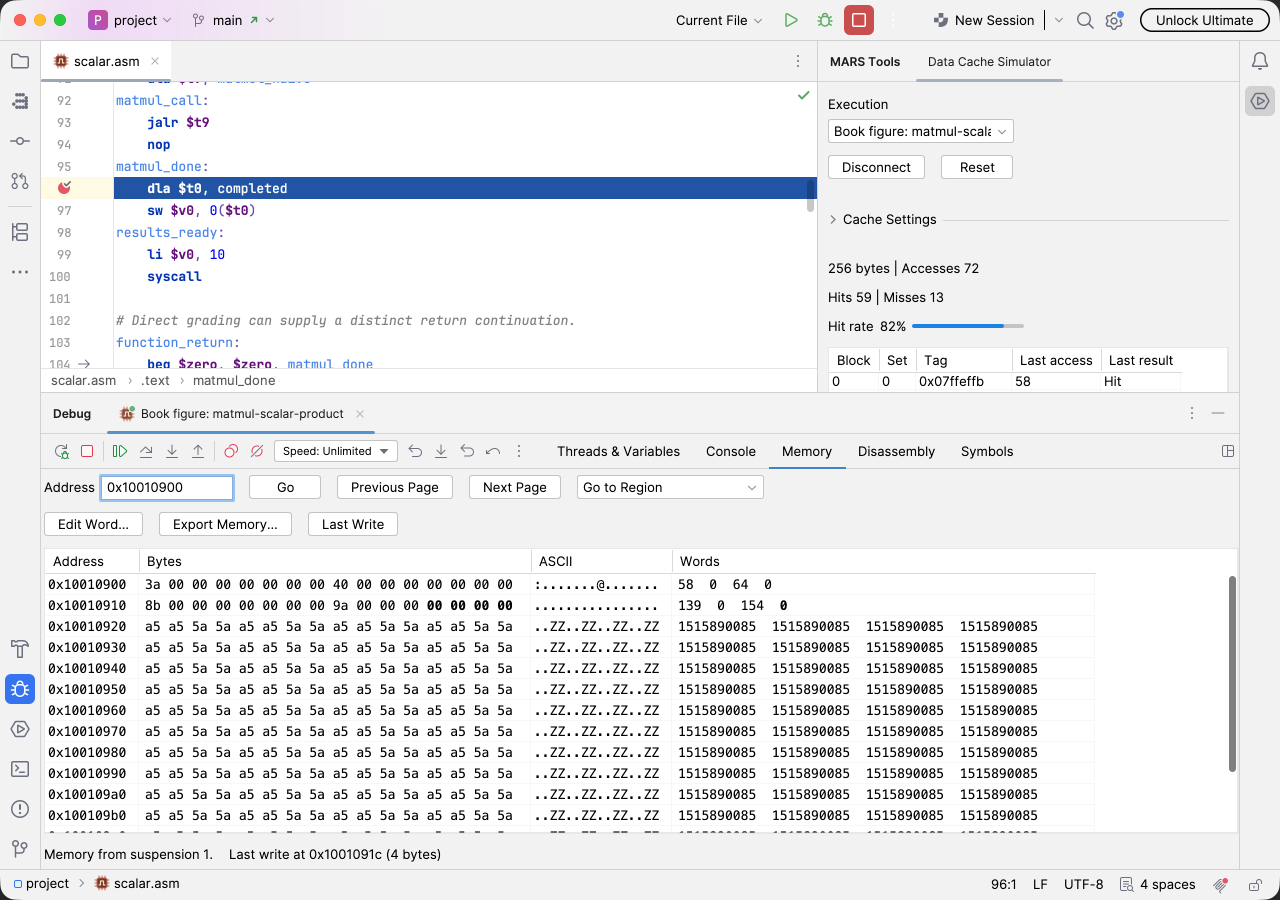
\includegraphics[width=0.84\linewidth,artifact,trim={\MARSmatmulscalarproductLeft{} \MARSmatmulscalarproductBottom{} \MARSmatmulscalarproductRight{} \MARSmatmulscalarproductTop{}},clip]{packages/022-blocked-matmul/captures/f01/product.png}};
\begin{scope}[shift={(product.south west)},x={($(product.south east)-(product.south west)$)},y={($(product.north west)-(product.south west)$)}]
\draw[black,line width=0.7pt] (0.194672131,0.055555556) rectangle (0.997950820,0.638888889);
\node[draw=black,fill=white,circle,inner sep=1.5pt,font=\footnotesize] at ($(0,0.638888889)+(-3mm,0)$) {5};
\end{scope}
\node[anchor=north west,inner sep=0,font=\small\bfseries] (caller-title) at ([yshift=-1mm]product.south west) {Shape, method and saved count};
\node[anchor=north west,inner sep=0] (caller) at ([yshift=-1mm]caller-title.south west) {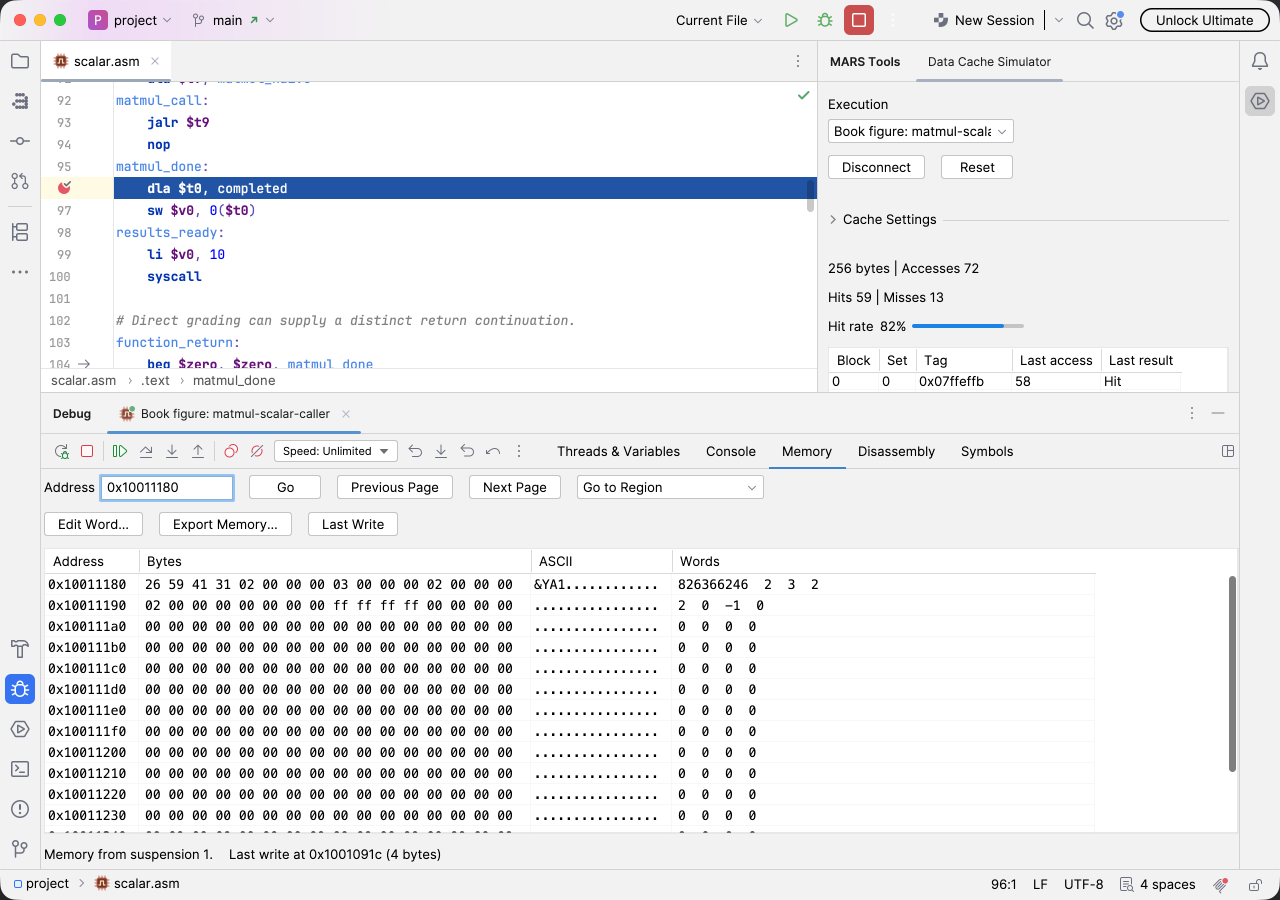
\includegraphics[width=0.84\linewidth,artifact,trim={\MARSmatmulscalarcallerLeft{} \MARSmatmulscalarcallerBottom{} \MARSmatmulscalarcallerRight{} \MARSmatmulscalarcallerTop{}},clip]{packages/022-blocked-matmul/captures/f01/caller.png}};
\begin{scope}[shift={(caller.south west)},x={($(caller.south east)-(caller.south west)$)},y={($(caller.north west)-(caller.south west)$)}]
\draw[black,line width=0.7pt] (0.194672131,0.055555556) rectangle (0.997950820,0.638888889);
\node[draw=black,fill=white,circle,inner sep=1.5pt,font=\footnotesize] at ($(0,0.638888889)+(-3mm,0)$) {6};
\end{scope}
\end{tikzpicture}
\par\smallskip
\begin{minipage}{\linewidth}
\small
\begin{enumerate}
\setlength{\itemsep}{2pt}
\setlength{\parsep}{0pt}
\item The next instruction at \texttt{matmul\_done} begins the caller\textquotesingle s result publication. The function has returned; the store to \texttt{completed} has not executed.
\item \texttt{v0 = 4} counts result cells, not bytes. Four doublewords occupy 32 bytes. The same shape has six words in each input matrix.
\item Left input begins at \texttt{0x10010000}. Its packed row-major words are $(1,2,3)$ and $(4,5,6)$; the last two words shown are padding.
\item Right input begins at \texttt{0x10010480}. Its rows are $(7,8)$, $(9,10)$ and $(11,12)$. A column advances by two words, while a left row advances by one.
\item At \texttt{0x10010900}, each eight-byte result contains a low word followed by its high word. The rows are $(58,64)$ and $(139,154)$, including $58=1\cdot7+2\cdot9+3\cdot11$. These positive results have zero high words.
\item The guard at \texttt{0x10011180} precedes the shape $M=2,K=3,N=2,T=2$. Method is zero and \texttt{completed} at \texttt{0x10011198} is still $-1$ (\texttt{ff ff ff ff}). Only the caller will replace it with four.
\end{enumerate}
\end{minipage}
\caption{The scalar function has returned four exact cells before the caller stores its count.}
\label{capture:022-blocked-matmul-f01}
\label{matmul-f01}
\end{figure}
\par
